\section{3DGM: 3D Gaussian Mapping}
\label{sec:gaussianmapping}
% \vspace{-2mm}
\subsection{Problem Formulation}
\paragraph{Assumption} We make reasonable assumptions about the stability of the environment and the transience of objects within it. Specifically, we assume that there are no major environmental changes, a realistic expectation when data is collected over a certain period under consistent weather and lighting conditions. Meanwhile, we consider all movable objects to be transient; despite their potential static nature during a particular traversal, they are expected to eventually move somewhere else, allowing the camera to capture dissensus over time. 
% \vspace{-3mm}
\paragraph{Setup} 
We conduct offline mapping of a specified spatial area by repeatedly traversing it with vehicles equipped with a monocular camera. The 3D environment map is represented by a set of 3D Gaussians, denoted as $\mathbf{G}=\{\mathbf{G}_i \mid i = 1, \ldots, N\}$. Each $\mathbf{G}_i$ has a set of learnable parameters $[\boldsymbol{\mu}_i, \mathbf{q}_i, \mathbf{s}_i, \alpha_i, \bm{\beta}_i, \mathbf{f}_i]$, where  \( \mathbf{f}_i \in \mathbb{R}^d \) is a self-supervised $d$-dimensional semantic feature such as DINO~\cite{oquab2023dinov2} for a more robust representation, and other parameters follow 3DGS as detailed in Sec.~\ref{sec:3dgs}. This mapping approach not only captures the geometry but also the photometry of the environment, yielding a comprehensive scene representation for downstream tasks such as geometry reconstruction and view synthesis. The input to our approach comes from a set of unposed images, sourced from multitraverse RGB videos, denoted by $\mathbf{I}=\{\mathbf{I}_t \in \mathbb{R}^{w\times h\times 3} \mid t = 1, \ldots, T\}$, where $T$ is the total number of images, $w$ and $h$ are the width and height of each image, respectively. 
% \vspace{-2mm}
\paragraph{Target} The target is to refine $\mathbf{G}$ to a level where it can accurately render images $\mathbf{I}_t(\boldsymbol{\xi}_t;\mathbf{G})$ that closely match the real images $\mathbf{I}_t$, captured from specific poses $\boldsymbol{\xi}_t$. Although $\mathbf{G}$ represents a 3D spatial map, the input images encompass 4D information with both spatial and temporal dimensions. Hence, our method needs to adeptly differentiate between the environment and ephemeral objects, like pedestrians and vehicles, to maintain robustness against pixels that represent transient entities. This necessitates addressing a robust estimation problem, where the outliers are transient objects—those that are either in motion or capable of moving—while the inliers are backgrounds.
% \vspace{-2mm}

\subsection{Overall Architecture}
Figure~\ref{fig:overall} shows our overall workflow. Given RGB images $\mathbf{I}$ collected across multiple traversals, we first leverage the classic Structure from Motion (SfM)~\cite{schonberger2016structure} to jointly reconstruct sparse points for the initialization of Gaussians and obtain the camera poses $\boldsymbol{\xi} = \{\boldsymbol{\xi}_t \mid t = 1, \ldots, T\}$. We then utilize the differential rendering pipeline of 3DGS to learn the positions, rotations, scales, opacities, colors, and semantic features of the 3D environmental Gaussians $\mathbf{G}$, supervised by ground truth RGB $\mathbf{I}$ and self-supervised feature maps~\cite{oquab2023dinov2} denoted by $\mathbf{F}=\{\mathbf{F}_t \in \mathbb{R}^{w\times h\times d} \mid t = 1, \ldots, T\}$. Then we exploit the feature residual maps to extract ephemeral object masks denoted by $\mathbf{M}=\{\mathbf{M}_t \in \mathbb{R}^{w\times h} \mid t = 1, \ldots, T\}$. Finally, we finetune 3D Gaussians $\mathbf{G}$ through robust differentiable rendering by leveraging the ephemerality masks. In summary, \texttt{3DGM} includes the three stages denoted by \texttt{Initialization}, \texttt{EmerSeg}, and \texttt{EnvGS}, as shown in Appendix~\ref{subsec:workflow-appendix}. We  detail each stage from Sec.~\ref{subsec:stage1} to~\ref{subsec:stage3}.

\begin{figure}[t]
\begin{center}
\centerline{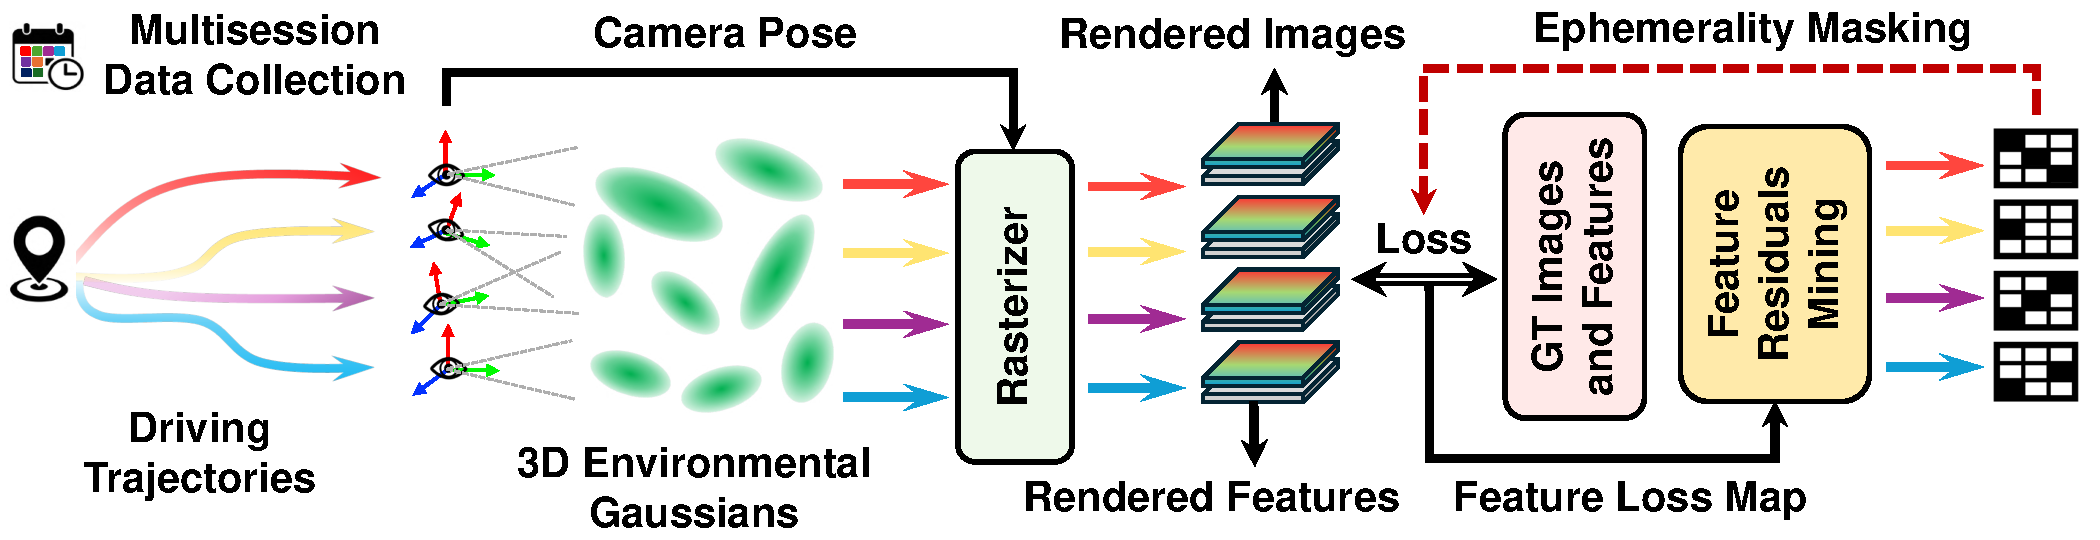
\includegraphics[width=\columnwidth]{figs_compressed/overview_compressed.pdf}}
\vspace{3mm}
\caption{\textbf{An overall illustration of \texttt{3DGM}.} Given RGB camera observations collected at different times, we use COLMAP to obtain the camera poses and initial Gaussian points. Then we utilize splatting-based rasterization to render both RGB images and robust features from the environmental Gaussians. We further leverage feature residuals to extract the object masks by mining spatial information of the residuals. Finally, we utilize the ephemerality masks to finetune the 3D Gaussians. }
\label{fig:overall}
\end{center}
\vspace{-5mm}
\end{figure}

\subsection{\texttt{Initialization}: Structure from Motion}
\label{subsec:stage1}
The SfM pipeline frequently faces challenges in single-traversal scenarios, largely due to the limited scene coverage achieved with RGB observations collected along a narrow and long camera trajectory. Conversely, RGB images from multiple traversals offer a broader array of viewpoints, significantly improving the triangulation and bundle adjustment processes. Additionally, this approach can leverage the 2D consensus of hand-crafted features in the correspondence search, providing inherent robustness against transient objects, which manifest as dissensus pixels across traversals. Moreover, our empirical experiments underscore the importance of the number of traversals for smooth initialization. A reduction in traversals can lead to a lack of sufficient image data, thereby failing the SfM initialization.

\subsection{\texttt{EmerSeg}: Emerged Ephemerality Segmentation by Feature Residuals Mining}
\label{subsec:stage2}
\paragraph{Feature distillation}
We utilize robust feature representations to enhance consensus verification, as the feature space exhibits better robustness against lighting variations and embodies semantic meanings, facilitating the decomposition of the transient objects by removing groups of semantically dissensus pixels.  We minimize the following RGB and feature rendering loss:
\begin{equation}
\mathcal{L} = \sum_t (\mathcal{L}_{rgb} ( \mathbf{I}_t(\boldsymbol{\xi}_t;\mathbf{G}) , \mathbf{I}_t ) + \mathcal{L}_{feat} ( \mathbf{F}_t(\boldsymbol{\xi}_t;\mathbf{G}) , \mathbf{F}_t ))
\end{equation}
where $\mathbf{I}_t(\boldsymbol{\xi}_t; \mathbf{G}) \in \mathbb{R}^{w\times h\times 3}$ and $\mathbf{F}_t(\boldsymbol{\xi}_t; \mathbf{G}) \in \mathbb{R}^{w\times h\times d}$ are the rendered RGB image and feature map given pose $\boldsymbol{\xi}_t \in \mathfrak{se}(3)$ and Gaussians $\mathbf{G}$. $\mathbf{I}_t$ and $\mathbf{F}_t$ are the corresponding ground truth RGB and feature map. $\mathcal{L}_{rgb}$ and $\mathcal{L}_{feat}$ are loss functions for RGB images and semantic features. \textit{As inlier pixels substantially outweigh outlier pixels, the model is primarily steered by gradients from consensus inlier pixels towards learning permanent features. As a result, pixels manifesting high loss in feature space are very likely to be outliers.}


\paragraph{Feature residuals mining} We derive transient object masks by leveraging the spatial information in the feature residual maps, as shown in the right column of Fig.~\ref{fig:vegas-loc1}\textasciitilde\ref{fig:vegas-loc6}. After training, we normalize the feature residuals and suppress pixels with residual values below a predefined threshold. Contours are then extracted from the normalized residual maps using spatial gradient information~\cite{suzuki1985topological}. We refine these contours by applying spatial priors to eliminate those that are too small or located in the sky. Finally, we merge nearby contours and extract a convex hull for each merged contour. Ultimately, ephemerality masks $\mathbf{M}$ are produced from simple postprocessing of feature residuals without additional training. More details are shown in Appendix~\ref{subsec:mining-appendix}.


\subsection{\texttt{EnvGS}: Environmental Gaussian Splatting via Robust Optimization}
\label{subsec:stage3}
After obtaining ephemerality masks $\mathbf{M}$, we focus on minimizing the following robust loss function (taking L1 loss as an example):
\begin{equation}
\mathcal{L} = \sum_t \mathcal{L}_{rgb} (  \mathbf{M}_t \odot \mathbf{I}_t(\boldsymbol{\xi}_t;\mathbf{G}) , \mathbf{M}_t \odot \mathbf{I}_t )
\end{equation}
where $\mathbf{M}_t$ is an ephemerality mask for the $t$-th image to downgrade the influence of outlier pixels. Optionally, we employ a depth smoothness loss and sky masks to further improve the geometry reconstruction, as illustrated in Appendix~\ref{subsec:addloss-appendix}.


\subsection{Comparison to Arts}
The pioneering work addressing similar problems is NeRF-W\cite{martin2021nerf}, which learns volumetric representations from unconstrained photo collections. It employs uncertainty estimation to mask transient objects situated in image areas of high uncertainty. The following research efforts propose to learn a transient mask, aiming to eliminate occluders\cite{chen2022hallucinated,yang2023cross}. Another related work is RobustNeRF~\cite{sabour2023robustnerf} which models distractors in training data as outliers of an optimization problem and proposes a form of robust estimation for NeRF training. 

We have three main differences from prior works.
\begin{itemize}[leftmargin=1.3em]
    \item \textbf{{Target problem}}\quad We formulate robotic multitraverse RGB mapping as a robust differentiable rendering problem, unlike previous works that focus on object-centric neural rendering of outdoor landmarks or multiple objects in indoor scenarios. 
    \item \textbf{{Scene decomposition}}\quad Our method enables a clearer decomposition of foreground and background, producing both 2D segmentation and 3D environmental Gaussians without any supervision. This represents a significant improvement over previous methods, which produce only blurry results in outdoor scenarios.
    \item \textbf{{Technical novelty}}\quad We use Gaussian Splatting instead of the conventional NeRF approach. Our robust feature distillation and feature residuals mining fully exploit the spatial information of the rendering loss map, resulting in much better ephemerality segmentation.
\end{itemize}




